% Enhanced FUR results on OpenBookQA with Llama-3.2-3B-Instruct
% Compiler: pdflatex
% Images used:
%   - overall_metrics_comparison.png
%   - recovery_cost_tradeoff.png
%   - example_1_508_step1_probabilities.png
%   - example_2_266_step3_probabilities.png
%   - efficacy_vs_answer_mass_shift.png
%   - full_fur_step_heatmap_top_instances.png

\documentclass[aspectratio=169,10pt]{beamer}

\usetheme{default}
\setbeamertemplate{navigation symbols}{}
\setbeamertemplate{footline}[frame number]
\setbeamertemplate{blocks}[default]

\usepackage[T1]{fontenc}
\usepackage{lmodern}
\usepackage{booktabs}
\usepackage{tabularx}
\usepackage{array}
\usepackage{graphicx}
\usepackage{xcolor}

\graphicspath{{./}}

\definecolor{mainblue}{RGB}{28,78,122}
\definecolor{accentred}{RGB}{178,54,48}

\setbeamercolor{frametitle}{fg=black,bg=white}
\setbeamerfont{frametitle}{series=\bfseries,size=\large}
\setbeamercolor{title}{fg=black}
\setbeamercolor{structure}{fg=mainblue}
\setbeamercolor{block title}{fg=black,bg=gray!12}
\setbeamercolor{block body}{fg=black,bg=white}

\newcommand{\good}[1]{\textcolor{mainblue}{\textbf{#1}}}
\newcommand{\warn}[1]{\textcolor{accentred}{\textbf{#1}}}

\title{Enhanced FUR: Selective Unlearning of Reasoning Steps}
\author{OpenBookQA + Llama-3.2-3B-Instruct}
\date{}

\begin{document}

\begin{frame}{Enhanced FUR: Experimental Setup}
\small
\begin{columns}[T,onlytextwidth]
  \begin{column}{0.48\textwidth}
    \textbf{Goal}

    \vspace{0.4em}
    Full FUR unlearns every CoT step, which is expensive.
    Enhanced FUR asks whether we can unlearn only a selected top-1 step and
    still recover many faithful cases found by Full FUR.

    \vspace{1em}
    \textbf{Compared methods}
    \begin{itemize}
      \item \textbf{Full FUR}: unlearn all segmented CoT steps.
      \item \textbf{Last-step top1}: unlearn only the final step.
      \item \textbf{Random top1}: unlearn one random step.
    \end{itemize}
  \end{column}

  \begin{column}{0.48\textwidth}
    \textbf{Run configuration}

    \vspace{0.3em}
    \begin{tabularx}{\linewidth}{p{0.44\linewidth}X}
      \toprule
      Model & Llama-3.2-3B-Instruct \\
      Dataset & OpenBookQA \\
      CoT cache & 100 generated CoTs \\
      Unlearning targets & 80 instances \\
      Specificity split & 20 held-out samples \\
      Method & NPO-KL, stepwise, sentencize \\
      Epochs / LR & 2 / 3e-05 \\
      Parallelism & 3 shards on A100 80GB \\
      \bottomrule
    \end{tabularx}

    \vspace{0.7em}
    \textbf{Note.} Llama-8B weights were gated at download time, so the complete
    run uses the locally available Llama-3B model.
  \end{column}
\end{columns}
\end{frame}

\begin{frame}{Overall Results: Full FUR vs. Selective Top-1}
\small
\begin{columns}[T,onlytextwidth]
  \begin{column}{0.50\textwidth}
    \textbf{Summary metrics}

    \vspace{0.25em}
    \scriptsize
    \begin{tabularx}{\linewidth}{>{\raggedright\arraybackslash}X r r r}
      \toprule
      Method & Rows & Faithful inst. & Specificity \\
      \midrule
      Full FUR & 431 & \warn{53/80 = 66.25\%} & 94.51\% \\
      Last top1 & 78 & 22/78 = 28.21\% & 94.74\% \\
      Random top1 & 71 & 21/71 = 29.58\% & 93.73\% \\
      \bottomrule
    \end{tabularx}

    \vspace{0.7em}
    \normalsize
    Full FUR finds many faithful instances, while top-1 variants use far fewer
    unlearning runs. All methods show high efficacy, around 89--90\%, and high
    specificity, around 94\%.
  \end{column}

  \begin{column}{0.50\textwidth}
    \centering
    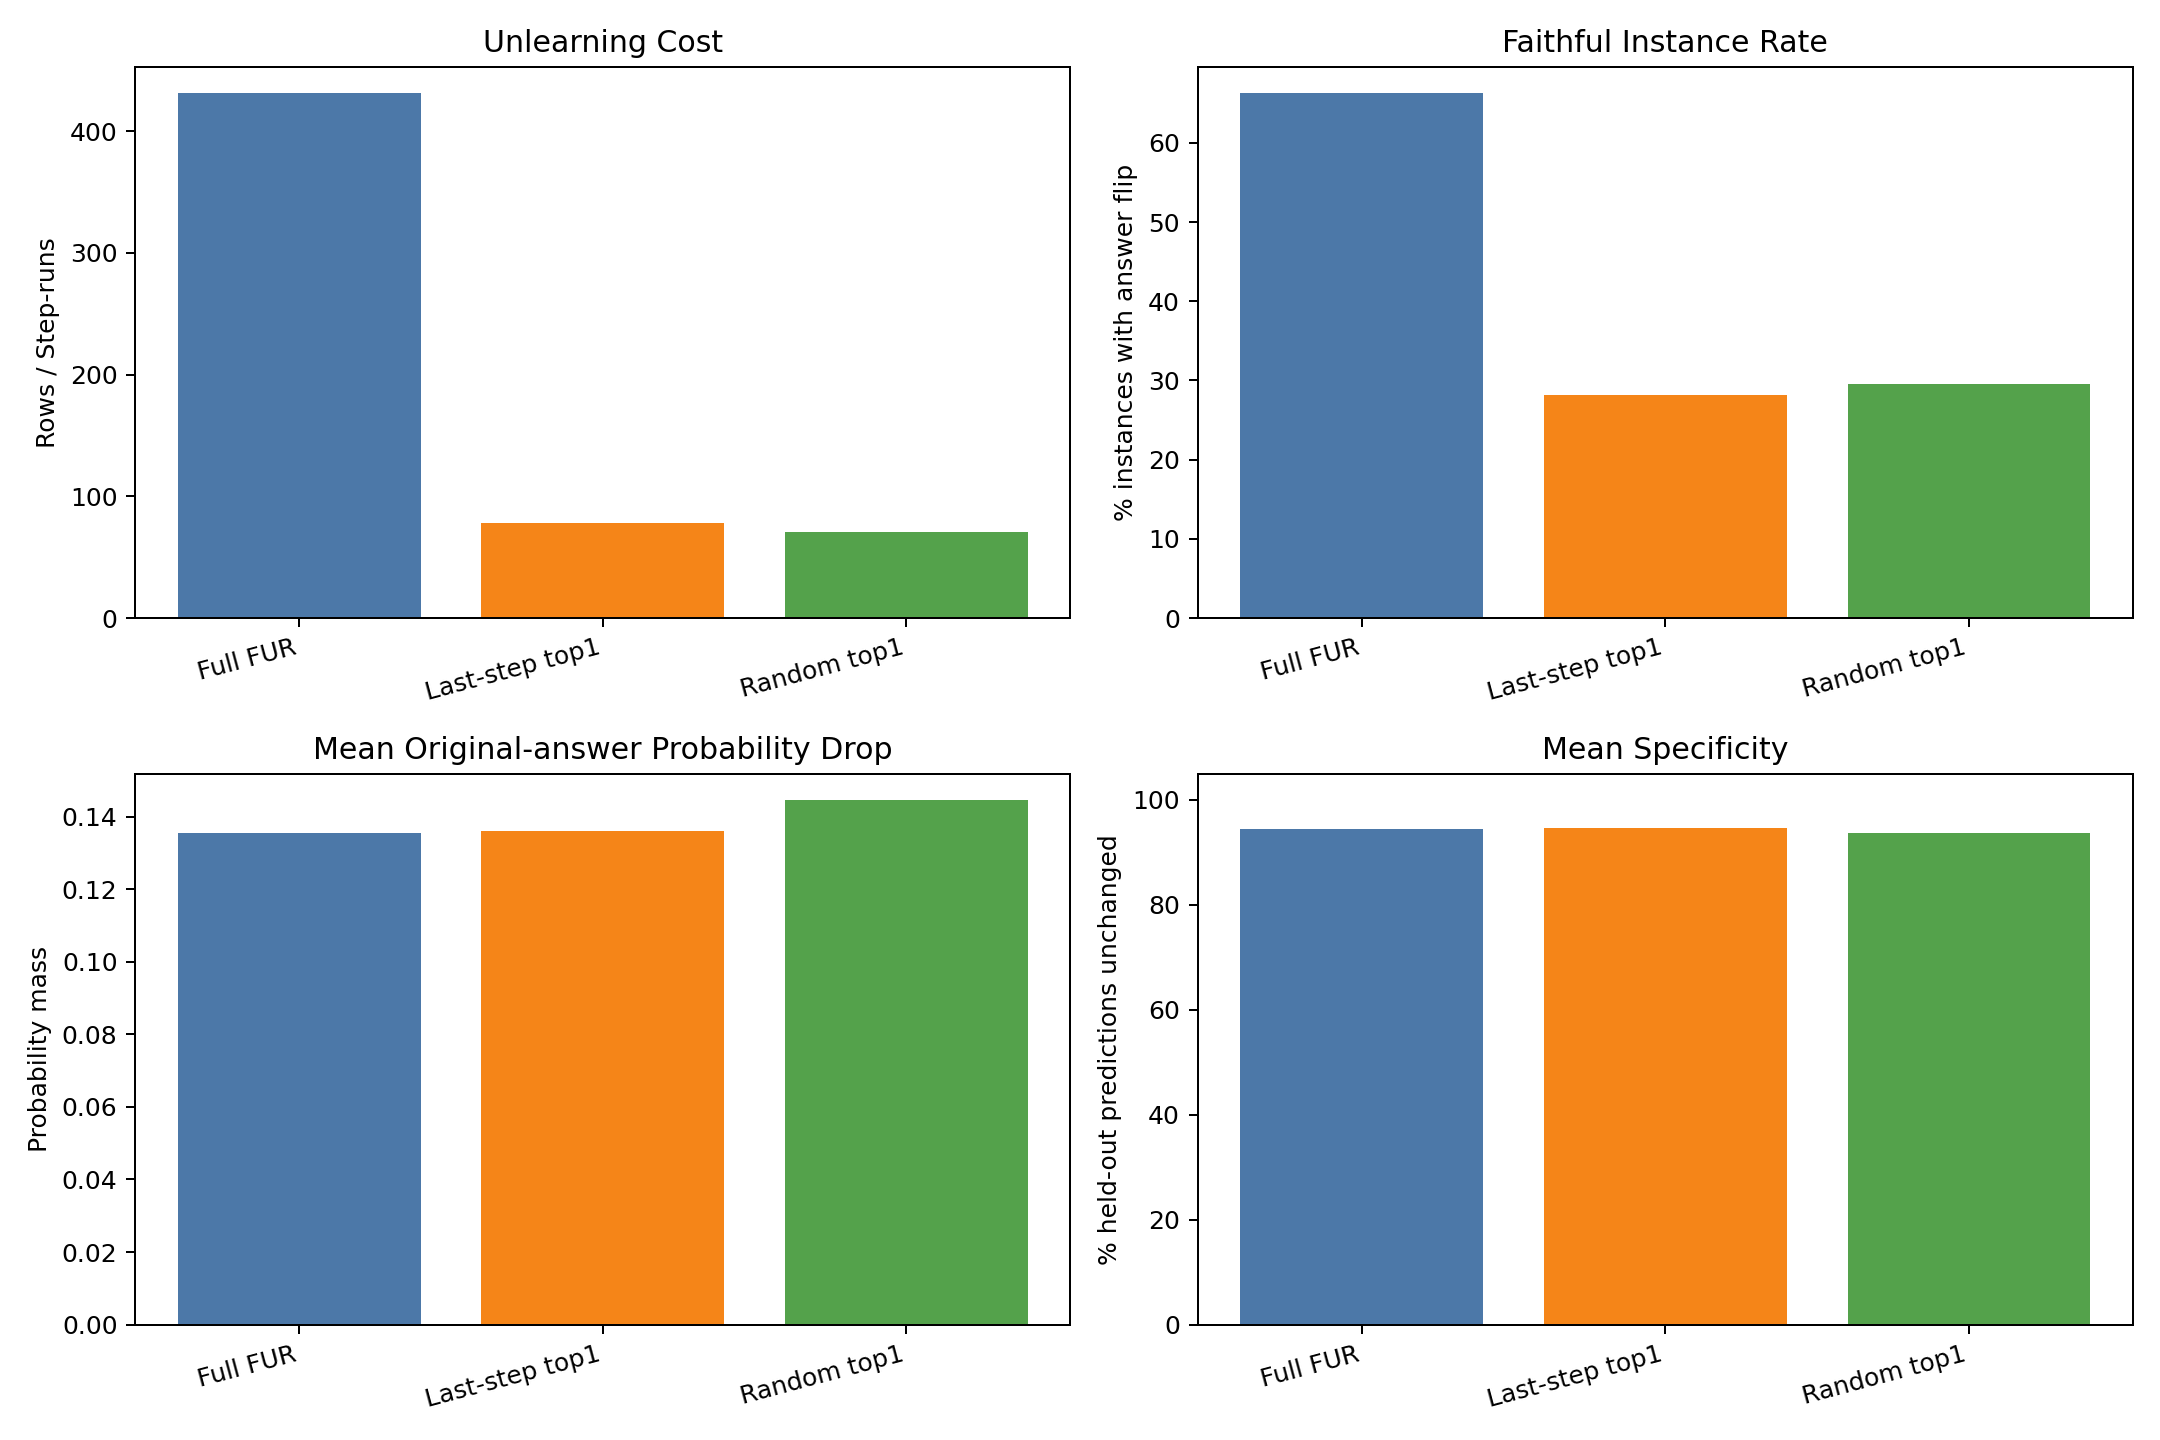
\includegraphics[width=\linewidth,height=0.78\textheight,keepaspectratio]{overall_metrics_comparison.png}
  \end{column}
\end{columns}
\end{frame}

\begin{frame}{Selective FUR: Recovery--Cost Tradeoff}
\small
\begin{columns}[T,onlytextwidth]
  \begin{column}{0.50\textwidth}
    \textbf{Recovery against Full FUR}

    \vspace{0.25em}
    \scriptsize
    \begin{tabularx}{\linewidth}{>{\raggedright\arraybackslash}X r r}
      \toprule
      Metric & Last top1 & Random top1 \\
      \midrule
      Cost reduction & \good{81.90\%} & \good{83.53\%} \\
      Faithful cases found & 22/53 & 21/53 \\
      Recovery@1 & 41.51\% & 39.62\% \\
      Step-Hit@1 & 17.21\% & 18.85\% \\
      Selected-step precision & 26.92\% & 32.39\% \\
      \bottomrule
    \end{tabularx}

    \vspace{0.7em}
    \normalsize
    Top-1 selective FUR is much cheaper, but the naive selectors miss many
    faithful steps. Last-step is not clearly better than random, suggesting that
    a real verifier/ranker is needed.
  \end{column}

  \begin{column}{0.50\textwidth}
    \centering
    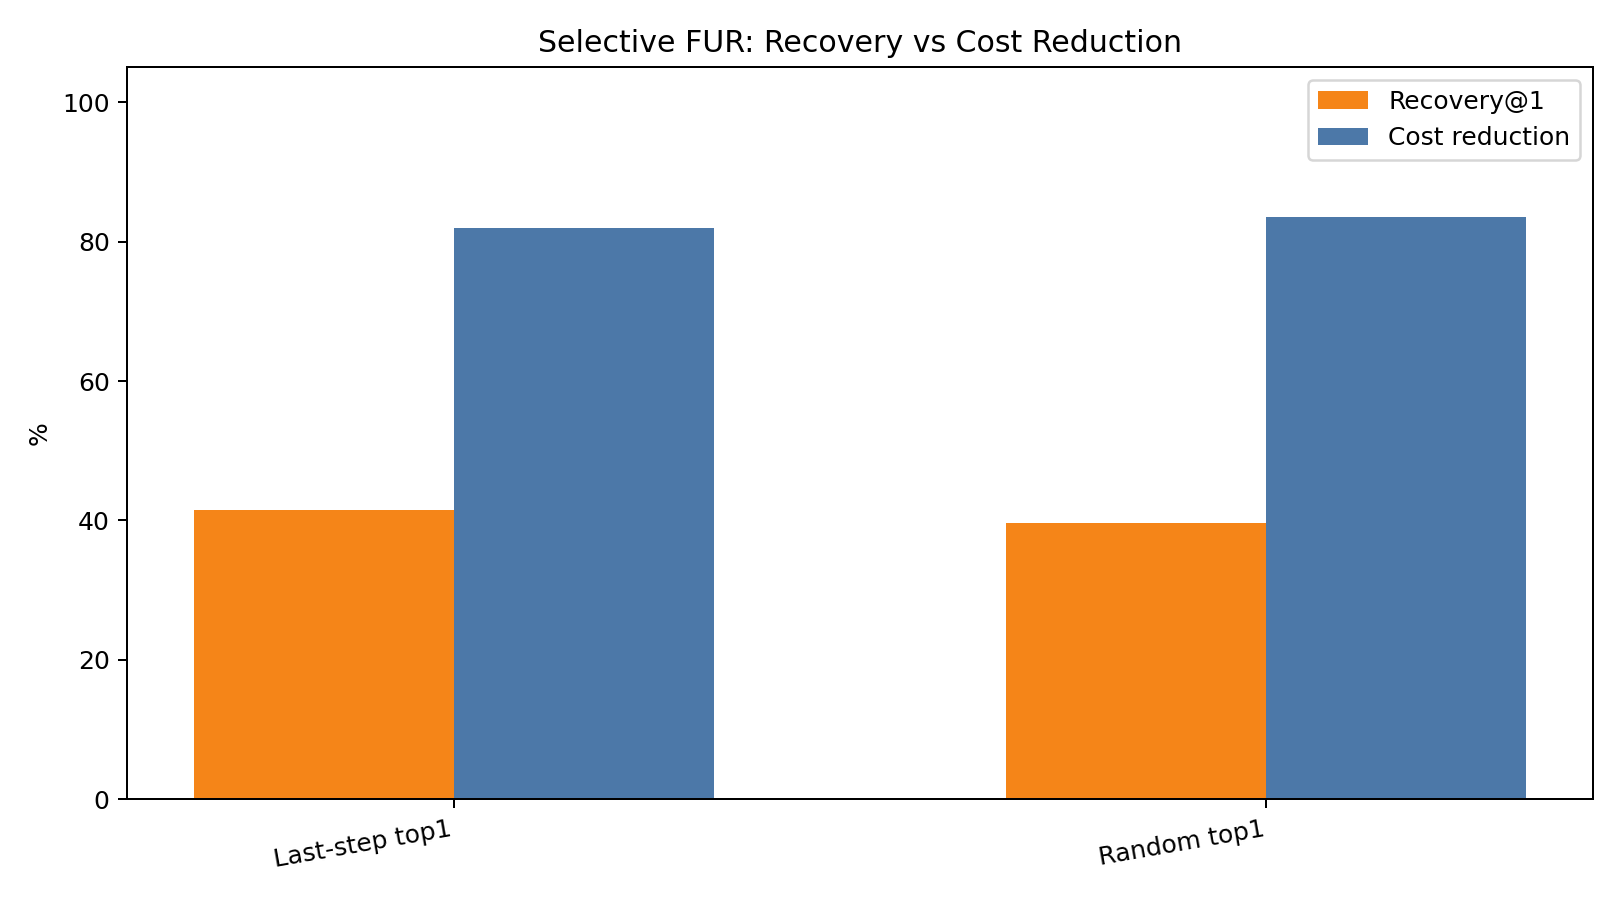
\includegraphics[width=\linewidth,height=0.78\textheight,keepaspectratio]{recovery_cost_tradeoff.png}
  \end{column}
\end{columns}
\end{frame}

\begin{frame}{Strong Positive Cases: Probability Transfer}
\small
\begin{columns}[T,onlytextwidth]
  \begin{column}{0.46\textwidth}
    \textbf{Largest Full-FUR answer shifts}

    \vspace{0.25em}
    \scriptsize
    \begin{tabularx}{\linewidth}{c c c r r}
      \toprule
      ID & Step & Change & Drop & Efficacy \\
      \midrule
      508 & 1 & D $\to$ A & 0.927 & 91.56\% \\
      266 & 3 & D $\to$ C & 0.926 & 96.09\% \\
      1189 & 1 & B $\to$ A & 0.925 & 92.04\% \\
      1577 & 7 & B $\to$ D & 0.900 & 95.81\% \\
      1577 & 11 & B $\to$ A & 0.894 & 97.16\% \\
      \bottomrule
    \end{tabularx}

    \vspace{0.7em}
    \normalsize
    These examples show the clearest causal effect: after one reasoning step is
    unlearned, the original answer probability almost vanishes and another option
    becomes dominant.
  \end{column}

  \begin{column}{0.27\textwidth}
    \centering
    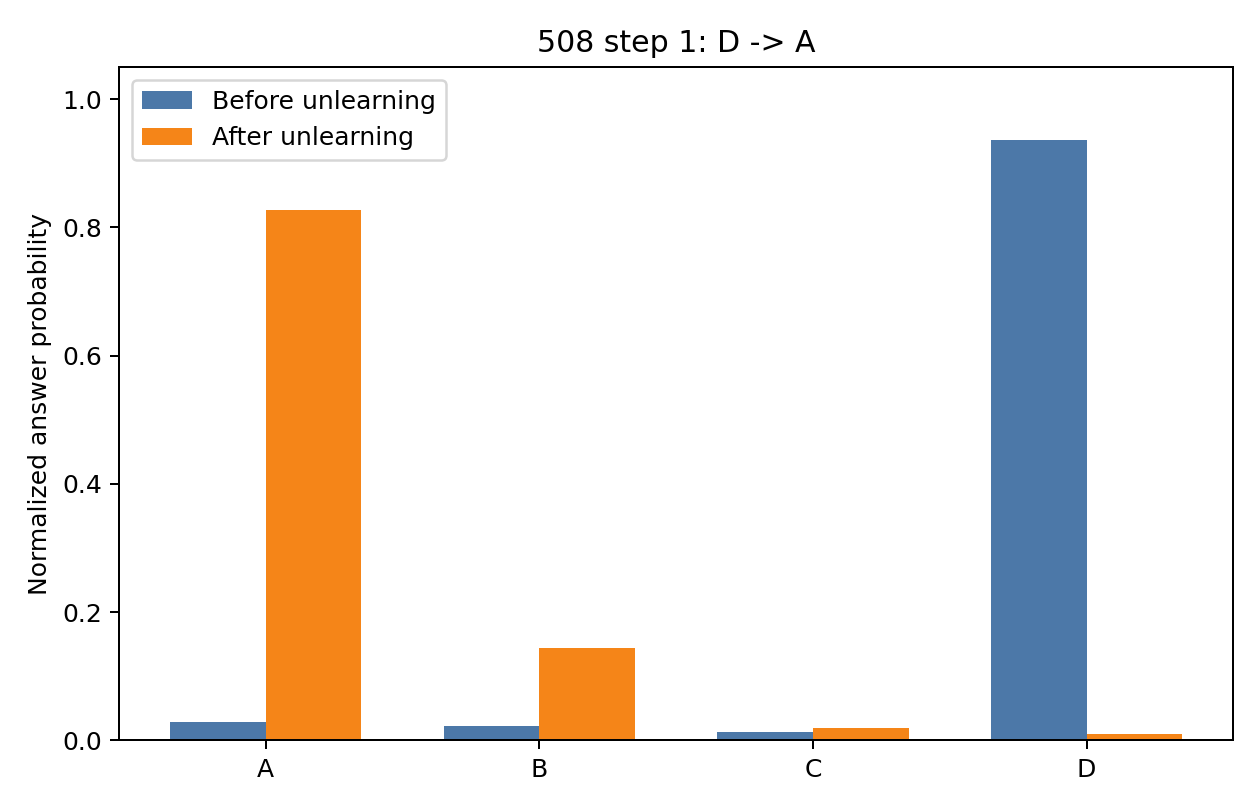
\includegraphics[width=\linewidth,height=0.70\textheight,keepaspectratio]{example_1_508_step1_probabilities.png}

    \vspace{0.2em}
    \scriptsize ID 508, step 1
  \end{column}

  \begin{column}{0.27\textwidth}
    \centering
    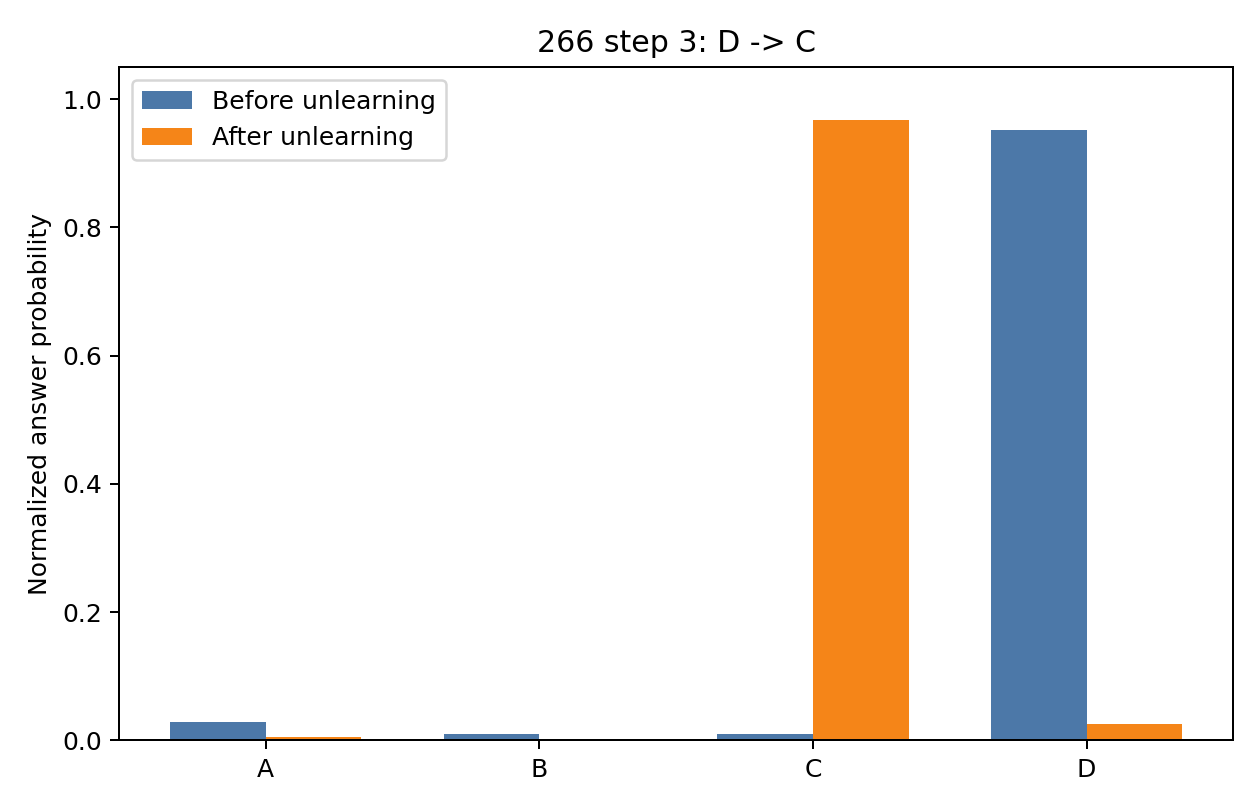
\includegraphics[width=\linewidth,height=0.70\textheight,keepaspectratio]{example_2_266_step3_probabilities.png}

    \vspace{0.2em}
    \scriptsize ID 266, step 3
  \end{column}
\end{columns}
\end{frame}

\begin{frame}{Global Pattern and Final Takeaways}
\begin{columns}[T,onlytextwidth]
  \begin{column}{0.50\textwidth}
    \centering
    \textbf{Efficacy vs. answer probability shift}

    \vspace{0.25em}
    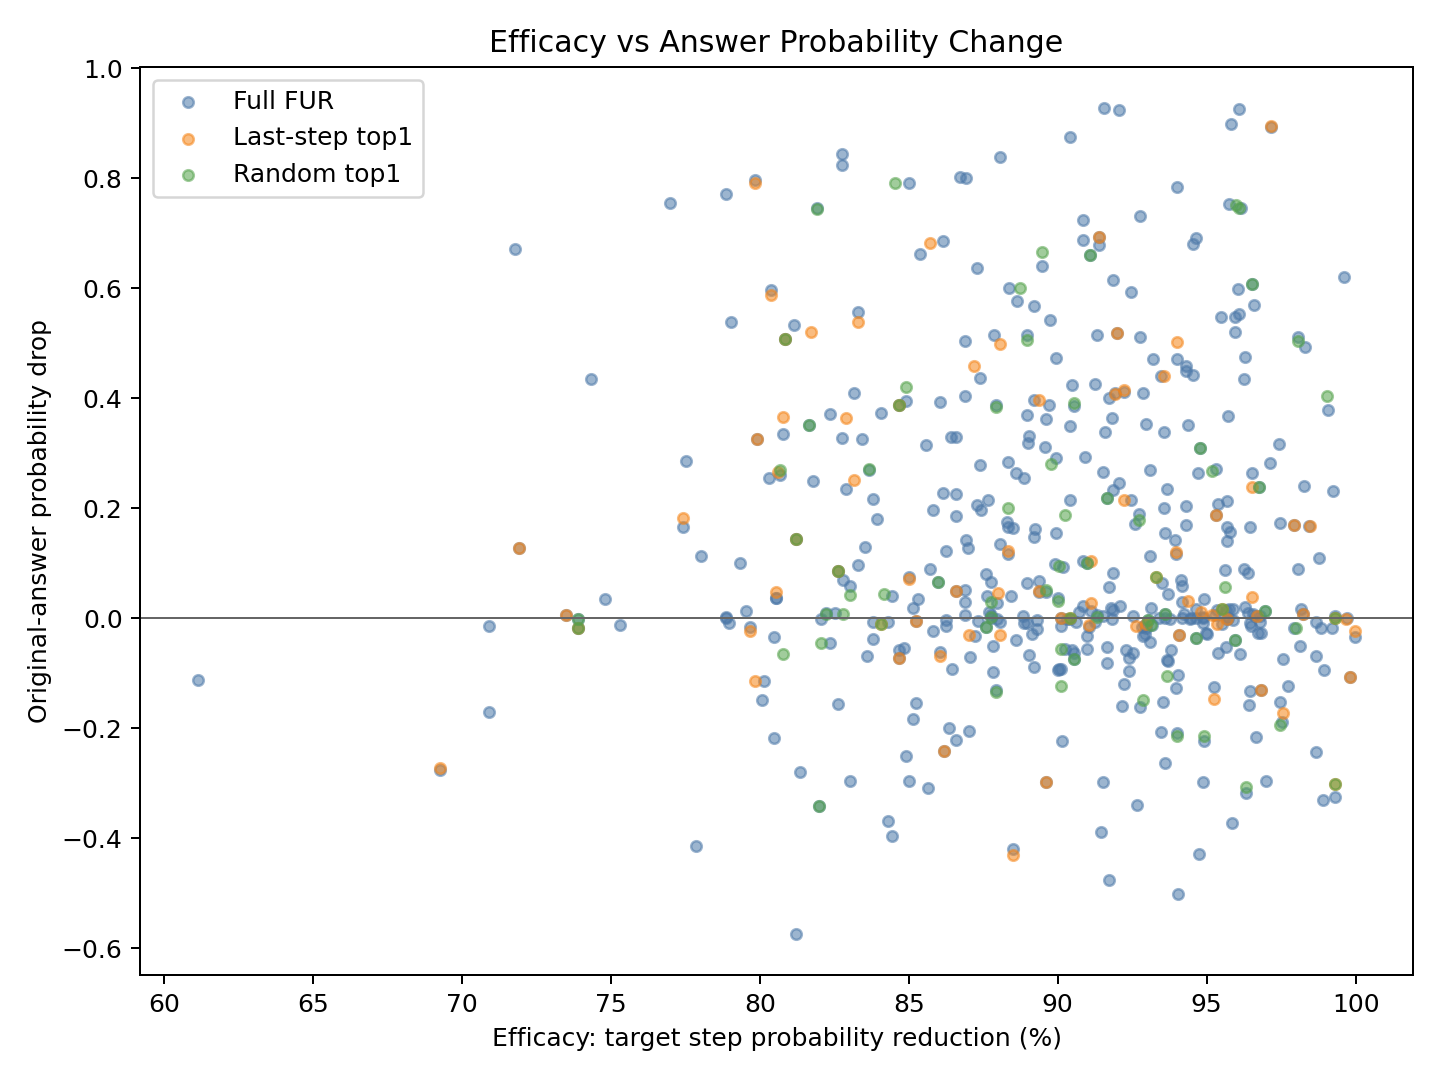
\includegraphics[width=\linewidth,height=0.55\textheight,keepaspectratio]{efficacy_vs_answer_mass_shift.png}
  \end{column}

  \begin{column}{0.50\textwidth}
    \centering
    \textbf{Full-FUR step salience}

    \vspace{0.25em}
    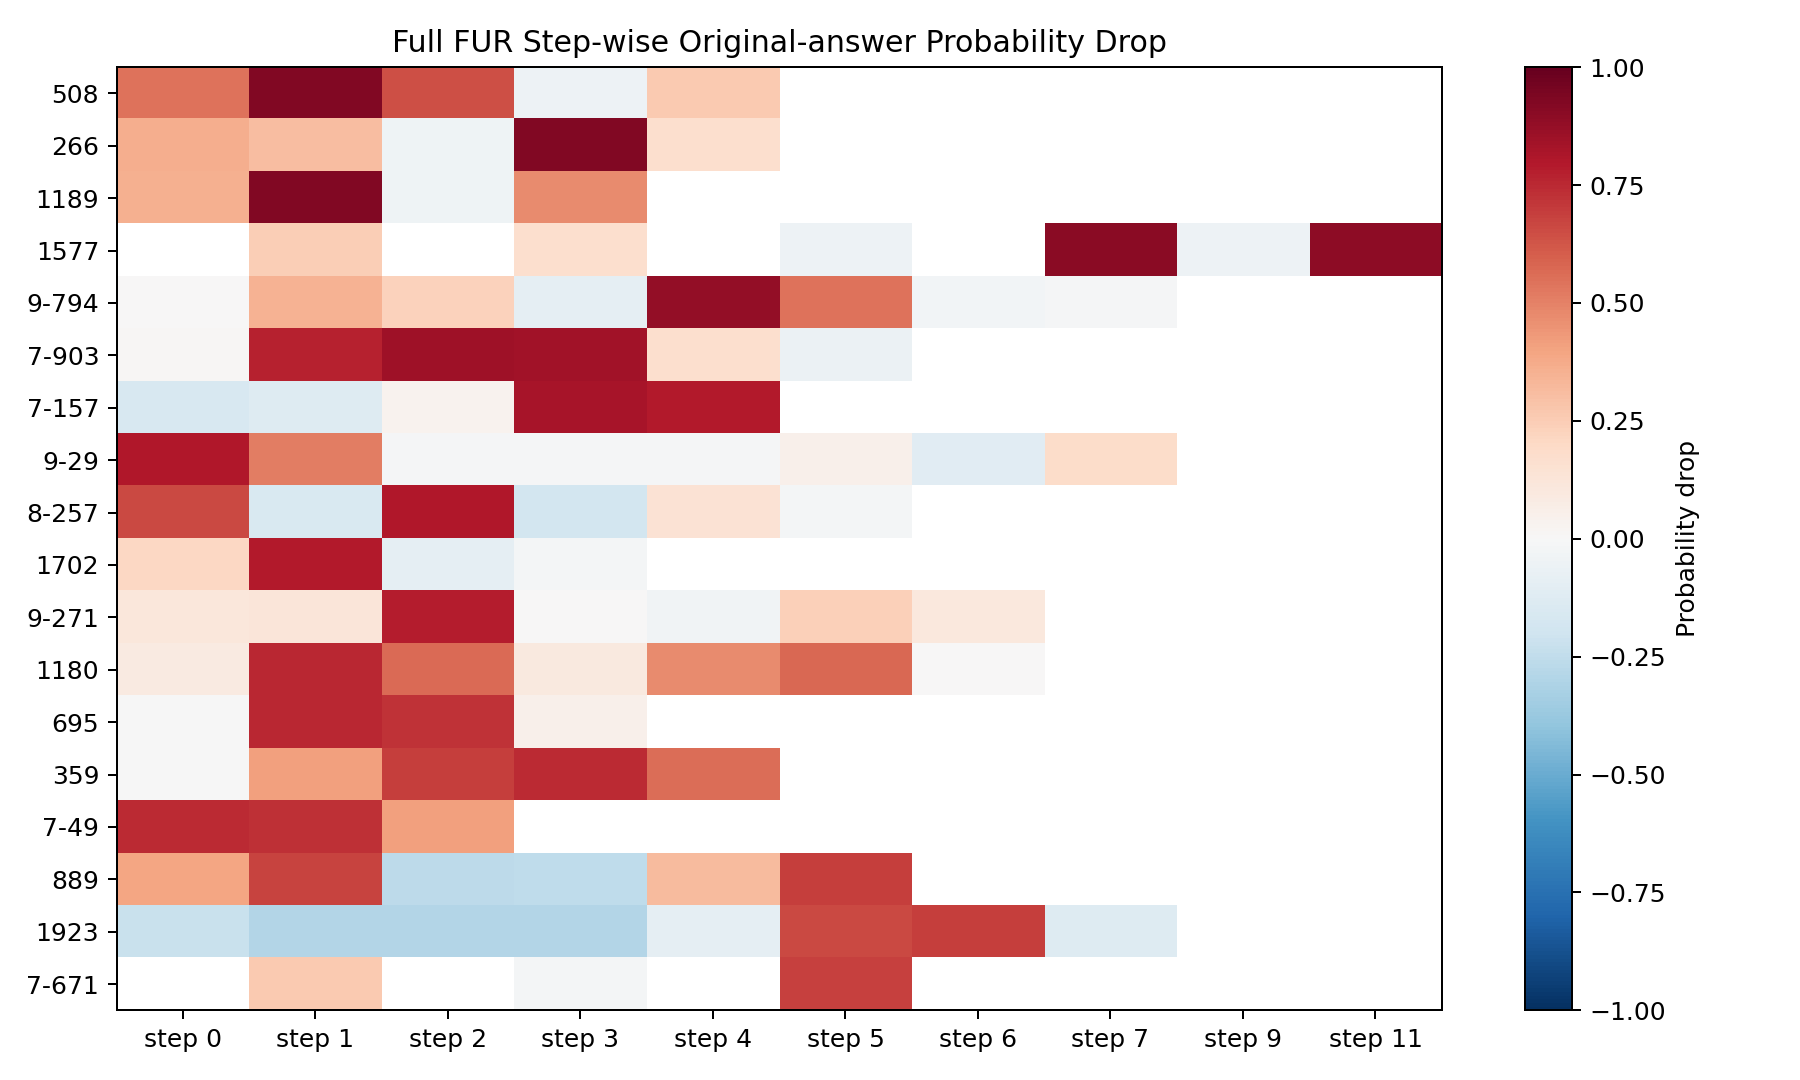
\includegraphics[width=\linewidth,height=0.55\textheight,keepaspectratio]{full_fur_step_heatmap_top_instances.png}
  \end{column}
\end{columns}

\vspace{0.25em}
\footnotesize
\begin{itemize}
  \item High efficacy does not guarantee an answer flip; probability-shift metrics are necessary.
  \item Full FUR is the best upper bound, but it is expensive: 431 step-runs for 80 instances.
  \item Top-1 selective FUR saves more than 80\% of the cost, but recovers only about 40\% of faithful instances.
  \item Next step: replace naive top-1 selection with deletion-based or verifier-guided ranking.
\end{itemize}
\end{frame}

\end{document}
